% Created by tikzDevice version 0.12.6 on 2026-07-09 15:42:25
% !TEX encoding = UTF-8 Unicode
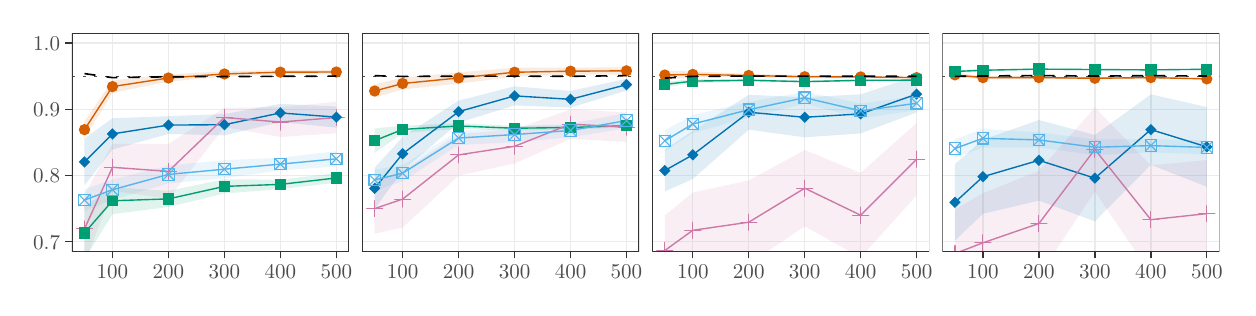
\begin{tikzpicture}[x=1pt,y=1pt]
\definecolor{fillColor}{RGB}{255,255,255}
\path[use as bounding box,fill=fillColor,fill opacity=0.00] (0,0) rectangle (433.62, 93.95);
\begin{scope}
\path[clip] (  0.00,  0.00) rectangle (433.62, 93.95);
\definecolor{drawColor}{RGB}{255,255,255}
\definecolor{fillColor}{RGB}{255,255,255}

\path[draw=drawColor,line width= 0.5pt,line join=round,line cap=round,fill=fillColor] ( -0.00,  0.00) rectangle (433.62, 93.95);
\end{scope}
\begin{scope}
\path[clip] ( 15.98, 12.99) rectangle (116.08, 91.95);
\definecolor{fillColor}{RGB}{255,255,255}

\path[fill=fillColor] ( 15.98, 12.99) rectangle (116.08, 91.95);
\definecolor{drawColor}{gray}{0.92}

\path[draw=drawColor,line width= 0.5pt,line join=round] ( 15.98, 16.58) --
	(116.08, 16.58);

\path[draw=drawColor,line width= 0.5pt,line join=round] ( 15.98, 40.50) --
	(116.08, 40.50);

\path[draw=drawColor,line width= 0.5pt,line join=round] ( 15.98, 64.43) --
	(116.08, 64.43);

\path[draw=drawColor,line width= 0.5pt,line join=round] ( 15.98, 88.36) --
	(116.08, 88.36);

\path[draw=drawColor,line width= 0.5pt,line join=round] ( 30.64, 12.99) --
	( 30.64, 91.95);

\path[draw=drawColor,line width= 0.5pt,line join=round] ( 50.87, 12.99) --
	( 50.87, 91.95);

\path[draw=drawColor,line width= 0.5pt,line join=round] ( 71.09, 12.99) --
	( 71.09, 91.95);

\path[draw=drawColor,line width= 0.5pt,line join=round] ( 91.31, 12.99) --
	( 91.31, 91.95);

\path[draw=drawColor,line width= 0.5pt,line join=round] (111.53, 12.99) --
	(111.53, 91.95);
\definecolor{drawColor}{gray}{0.30}

\path[draw=drawColor,line width= 0.4pt,dash pattern=on 1pt off 3pt ,line join=round] ( 15.98, 76.40) -- (116.08, 76.40);
\definecolor{fillColor}{RGB}{213,94,0}

\path[fill=fillColor,fill opacity=0.12] ( 20.53, 60.11) --
	( 30.64, 74.91) --
	( 50.87, 77.08) --
	( 71.09, 78.22) --
	( 91.31, 78.66) --
	(111.53, 78.59) --
	(111.53, 77.28) --
	( 91.31, 77.07) --
	( 71.09, 76.23) --
	( 50.87, 74.45) --
	( 30.64, 70.40) --
	( 20.53, 54.08) --
	cycle;

\path[] ( 20.53, 60.11) --
	( 30.64, 74.91) --
	( 50.87, 77.08) --
	( 71.09, 78.22) --
	( 91.31, 78.66) --
	(111.53, 78.59);

\path[] (111.53, 77.28) --
	( 91.31, 77.07) --
	( 71.09, 76.23) --
	( 50.87, 74.45) --
	( 30.64, 70.40) --
	( 20.53, 54.08);
\definecolor{fillColor}{RGB}{0,158,115}

\path[fill=fillColor,fill opacity=0.12] ( 20.53, 29.36) --
	( 30.64, 36.24) --
	( 50.87, 35.00) --
	( 71.09, 39.16) --
	( 91.31, 39.04) --
	(111.53, 41.36) --
	(111.53, 37.93) --
	( 91.31, 35.61) --
	( 71.09, 34.04) --
	( 50.87, 29.16) --
	( 30.64, 26.56) --
	( 20.53, 10.23) --
	cycle;

\path[] ( 20.53, 29.36) --
	( 30.64, 36.24) --
	( 50.87, 35.00) --
	( 71.09, 39.16) --
	( 91.31, 39.04) --
	(111.53, 41.36);

\path[] (111.53, 37.93) --
	( 91.31, 35.61) --
	( 71.09, 34.04) --
	( 50.87, 29.16) --
	( 30.64, 26.56) --
	( 20.53, 10.23);
\definecolor{fillColor}{RGB}{0,114,178}

\path[fill=fillColor,fill opacity=0.12] ( 20.53, 53.91) --
	( 30.64, 61.21) --
	( 50.87, 61.96) --
	( 71.09, 62.73) --
	( 91.31, 66.44) --
	(111.53, 65.46) --
	(111.53, 57.81) --
	( 91.31, 59.84) --
	( 71.09, 55.04) --
	( 50.87, 55.54) --
	( 30.64, 49.92) --
	( 20.53, 36.96) --
	cycle;

\path[] ( 20.53, 53.91) --
	( 30.64, 61.21) --
	( 50.87, 61.96) --
	( 71.09, 62.73) --
	( 91.31, 66.44) --
	(111.53, 65.46);

\path[] (111.53, 57.81) --
	( 91.31, 59.84) --
	( 71.09, 55.04) --
	( 50.87, 55.54) --
	( 30.64, 49.92) --
	( 20.53, 36.96);
\definecolor{fillColor}{RGB}{204,121,167}

\path[fill=fillColor,fill opacity=0.12] ( 20.53, 33.70) --
	( 30.64, 51.94) --
	( 50.87, 51.91) --
	( 71.09, 64.93) --
	( 91.31, 65.26) --
	(111.53, 67.16) --
	(111.53, 55.78) --
	( 91.31, 54.45) --
	( 71.09, 58.04) --
	( 50.87, 32.14) --
	( 30.64, 35.04) --
	( 20.53,  8.78) --
	cycle;

\path[] ( 20.53, 33.70) --
	( 30.64, 51.94) --
	( 50.87, 51.91) --
	( 71.09, 64.93) --
	( 91.31, 65.26) --
	(111.53, 67.16);

\path[] (111.53, 55.78) --
	( 91.31, 54.45) --
	( 71.09, 58.04) --
	( 50.87, 32.14) --
	( 30.64, 35.04) --
	( 20.53,  8.78);
\definecolor{fillColor}{RGB}{86,180,233}

\path[fill=fillColor,fill opacity=0.12] ( 20.53, 35.52) --
	( 30.64, 39.07) --
	( 50.87, 44.17) --
	( 71.09, 46.04) --
	( 91.31, 46.92) --
	(111.53, 49.30) --
	(111.53, 43.80) --
	( 91.31, 42.36) --
	( 71.09, 39.57) --
	( 50.87, 37.68) --
	( 30.64, 31.72) --
	( 20.53, 27.81) --
	cycle;

\path[] ( 20.53, 35.52) --
	( 30.64, 39.07) --
	( 50.87, 44.17) --
	( 71.09, 46.04) --
	( 91.31, 46.92) --
	(111.53, 49.30);

\path[] (111.53, 43.80) --
	( 91.31, 42.36) --
	( 71.09, 39.57) --
	( 50.87, 37.68) --
	( 30.64, 31.72) --
	( 20.53, 27.81);
\definecolor{drawColor}{RGB}{213,94,0}

\path[draw=drawColor,line width= 0.5pt,line join=round] ( 20.53, 57.10) --
	( 30.64, 72.66) --
	( 50.87, 75.77) --
	( 71.09, 77.22) --
	( 91.31, 77.87) --
	(111.53, 77.93);
\definecolor{drawColor}{RGB}{0,158,115}

\path[draw=drawColor,line width= 0.5pt,line join=round] ( 20.53, 19.79) --
	( 30.64, 31.40) --
	( 50.87, 32.08) --
	( 71.09, 36.60) --
	( 91.31, 37.32) --
	(111.53, 39.64);
\definecolor{drawColor}{RGB}{0,114,178}

\path[draw=drawColor,line width= 0.5pt,line join=round] ( 20.53, 45.44) --
	( 30.64, 55.56) --
	( 50.87, 58.75) --
	( 71.09, 58.89) --
	( 91.31, 63.14) --
	(111.53, 61.63);
\definecolor{drawColor}{RGB}{204,121,167}

\path[draw=drawColor,line width= 0.5pt,line join=round] ( 20.53, 21.24) --
	( 30.64, 43.49) --
	( 50.87, 42.02) --
	( 71.09, 61.48) --
	( 91.31, 59.85) --
	(111.53, 61.47);
\definecolor{drawColor}{RGB}{86,180,233}

\path[draw=drawColor,line width= 0.5pt,line join=round] ( 20.53, 31.67) --
	( 30.64, 35.39) --
	( 50.87, 40.93) --
	( 71.09, 42.81) --
	( 91.31, 44.64) --
	(111.53, 46.55);
\definecolor{fillColor}{RGB}{213,94,0}

\path[fill=fillColor] ( 20.53, 57.10) circle (  2.05);
\definecolor{drawColor}{RGB}{204,121,167}

\path[draw=drawColor,line width= 0.4pt,line join=round,line cap=round] ( 17.63, 21.24) -- ( 23.43, 21.24);

\path[draw=drawColor,line width= 0.4pt,line join=round,line cap=round] ( 20.53, 18.34) -- ( 20.53, 24.14);
\definecolor{fillColor}{RGB}{0,158,115}

\path[fill=fillColor] ( 18.48, 17.74) --
	( 22.58, 17.74) --
	( 22.58, 21.84) --
	( 18.48, 21.84) --
	cycle;
\definecolor{fillColor}{RGB}{0,114,178}

\path[fill=fillColor] ( 18.48, 45.44) --
	( 20.53, 47.49) --
	( 22.58, 45.44) --
	( 20.53, 43.39) --
	cycle;
\definecolor{drawColor}{RGB}{86,180,233}

\path[draw=drawColor,line width= 0.4pt,line join=round,line cap=round] ( 18.48, 29.61) rectangle ( 22.58, 33.72);

\path[draw=drawColor,line width= 0.4pt,line join=round,line cap=round] ( 18.48, 29.61) -- ( 22.58, 33.72);

\path[draw=drawColor,line width= 0.4pt,line join=round,line cap=round] ( 18.48, 33.72) -- ( 22.58, 29.61);
\definecolor{fillColor}{RGB}{213,94,0}

\path[fill=fillColor] ( 30.64, 72.66) circle (  2.05);
\definecolor{drawColor}{RGB}{204,121,167}

\path[draw=drawColor,line width= 0.4pt,line join=round,line cap=round] ( 27.74, 43.49) -- ( 33.55, 43.49);

\path[draw=drawColor,line width= 0.4pt,line join=round,line cap=round] ( 30.64, 40.59) -- ( 30.64, 46.39);
\definecolor{fillColor}{RGB}{0,158,115}

\path[fill=fillColor] ( 28.59, 29.35) --
	( 32.70, 29.35) --
	( 32.70, 33.45) --
	( 28.59, 33.45) --
	cycle;
\definecolor{fillColor}{RGB}{0,114,178}

\path[fill=fillColor] ( 28.59, 55.56) --
	( 30.64, 57.61) --
	( 32.70, 55.56) --
	( 30.64, 53.51) --
	cycle;
\definecolor{drawColor}{RGB}{86,180,233}

\path[draw=drawColor,line width= 0.4pt,line join=round,line cap=round] ( 28.59, 33.34) rectangle ( 32.70, 37.44);

\path[draw=drawColor,line width= 0.4pt,line join=round,line cap=round] ( 28.59, 33.34) -- ( 32.70, 37.44);

\path[draw=drawColor,line width= 0.4pt,line join=round,line cap=round] ( 28.59, 37.44) -- ( 32.70, 33.34);
\definecolor{fillColor}{RGB}{213,94,0}

\path[fill=fillColor] ( 50.87, 75.77) circle (  2.05);
\definecolor{drawColor}{RGB}{204,121,167}

\path[draw=drawColor,line width= 0.4pt,line join=round,line cap=round] ( 47.96, 42.02) -- ( 53.77, 42.02);

\path[draw=drawColor,line width= 0.4pt,line join=round,line cap=round] ( 50.87, 39.12) -- ( 50.87, 44.92);
\definecolor{fillColor}{RGB}{0,158,115}

\path[fill=fillColor] ( 48.81, 30.03) --
	( 52.92, 30.03) --
	( 52.92, 34.13) --
	( 48.81, 34.13) --
	cycle;
\definecolor{fillColor}{RGB}{0,114,178}

\path[fill=fillColor] ( 48.81, 58.75) --
	( 50.87, 60.80) --
	( 52.92, 58.75) --
	( 50.87, 56.70) --
	cycle;
\definecolor{drawColor}{RGB}{86,180,233}

\path[draw=drawColor,line width= 0.4pt,line join=round,line cap=round] ( 48.81, 38.87) rectangle ( 52.92, 42.98);

\path[draw=drawColor,line width= 0.4pt,line join=round,line cap=round] ( 48.81, 38.87) -- ( 52.92, 42.98);

\path[draw=drawColor,line width= 0.4pt,line join=round,line cap=round] ( 48.81, 42.98) -- ( 52.92, 38.87);
\definecolor{fillColor}{RGB}{213,94,0}

\path[fill=fillColor] ( 71.09, 77.22) circle (  2.05);
\definecolor{drawColor}{RGB}{204,121,167}

\path[draw=drawColor,line width= 0.4pt,line join=round,line cap=round] ( 68.19, 61.48) -- ( 73.99, 61.48);

\path[draw=drawColor,line width= 0.4pt,line join=round,line cap=round] ( 71.09, 58.58) -- ( 71.09, 64.39);
\definecolor{fillColor}{RGB}{0,158,115}

\path[fill=fillColor] ( 69.04, 34.55) --
	( 73.14, 34.55) --
	( 73.14, 38.65) --
	( 69.04, 38.65) --
	cycle;
\definecolor{fillColor}{RGB}{0,114,178}

\path[fill=fillColor] ( 69.04, 58.89) --
	( 71.09, 60.94) --
	( 73.14, 58.89) --
	( 71.09, 56.83) --
	cycle;
\definecolor{drawColor}{RGB}{86,180,233}

\path[draw=drawColor,line width= 0.4pt,line join=round,line cap=round] ( 69.04, 40.76) rectangle ( 73.14, 44.86);

\path[draw=drawColor,line width= 0.4pt,line join=round,line cap=round] ( 69.04, 40.76) -- ( 73.14, 44.86);

\path[draw=drawColor,line width= 0.4pt,line join=round,line cap=round] ( 69.04, 44.86) -- ( 73.14, 40.76);
\definecolor{fillColor}{RGB}{213,94,0}

\path[fill=fillColor] ( 91.31, 77.87) circle (  2.05);
\definecolor{drawColor}{RGB}{204,121,167}

\path[draw=drawColor,line width= 0.4pt,line join=round,line cap=round] ( 88.41, 59.85) -- ( 94.21, 59.85);

\path[draw=drawColor,line width= 0.4pt,line join=round,line cap=round] ( 91.31, 56.95) -- ( 91.31, 62.75);
\definecolor{fillColor}{RGB}{0,158,115}

\path[fill=fillColor] ( 89.26, 35.27) --
	( 93.36, 35.27) --
	( 93.36, 39.37) --
	( 89.26, 39.37) --
	cycle;
\definecolor{fillColor}{RGB}{0,114,178}

\path[fill=fillColor] ( 89.26, 63.14) --
	( 91.31, 65.20) --
	( 93.36, 63.14) --
	( 91.31, 61.09) --
	cycle;
\definecolor{drawColor}{RGB}{86,180,233}

\path[draw=drawColor,line width= 0.4pt,line join=round,line cap=round] ( 89.26, 42.59) rectangle ( 93.36, 46.69);

\path[draw=drawColor,line width= 0.4pt,line join=round,line cap=round] ( 89.26, 42.59) -- ( 93.36, 46.69);

\path[draw=drawColor,line width= 0.4pt,line join=round,line cap=round] ( 89.26, 46.69) -- ( 93.36, 42.59);
\definecolor{fillColor}{RGB}{213,94,0}

\path[fill=fillColor] (111.53, 77.93) circle (  2.05);
\definecolor{drawColor}{RGB}{204,121,167}

\path[draw=drawColor,line width= 0.4pt,line join=round,line cap=round] (108.63, 61.47) -- (114.43, 61.47);

\path[draw=drawColor,line width= 0.4pt,line join=round,line cap=round] (111.53, 58.57) -- (111.53, 64.37);
\definecolor{fillColor}{RGB}{0,158,115}

\path[fill=fillColor] (109.48, 37.59) --
	(113.58, 37.59) --
	(113.58, 41.69) --
	(109.48, 41.69) --
	cycle;
\definecolor{fillColor}{RGB}{0,114,178}

\path[fill=fillColor] (109.48, 61.63) --
	(111.53, 63.68) --
	(113.58, 61.63) --
	(111.53, 59.58) --
	cycle;
\definecolor{drawColor}{RGB}{86,180,233}

\path[draw=drawColor,line width= 0.4pt,line join=round,line cap=round] (109.48, 44.50) rectangle (113.58, 48.60);

\path[draw=drawColor,line width= 0.4pt,line join=round,line cap=round] (109.48, 44.50) -- (113.58, 48.60);

\path[draw=drawColor,line width= 0.4pt,line join=round,line cap=round] (109.48, 48.60) -- (113.58, 44.50);
\definecolor{drawColor}{RGB}{0,0,0}

\path[draw=drawColor,line width= 0.6pt,dash pattern=on 4pt off 4pt ,line join=round] ( 20.53, 77.36) --
	( 30.64, 75.89) --
	( 50.87, 76.21) --
	( 71.09, 76.28) --
	( 91.31, 76.36) --
	(111.53, 76.46);
\definecolor{drawColor}{gray}{0.20}

\path[draw=drawColor,line width= 0.5pt,line join=round,line cap=round] ( 15.98, 12.99) rectangle (116.08, 91.95);
\end{scope}
\begin{scope}
\path[clip] (120.83, 12.99) rectangle (220.93, 91.95);
\definecolor{fillColor}{RGB}{255,255,255}

\path[fill=fillColor] (120.83, 12.99) rectangle (220.93, 91.95);
\definecolor{drawColor}{gray}{0.92}

\path[draw=drawColor,line width= 0.5pt,line join=round] (120.83, 16.58) --
	(220.93, 16.58);

\path[draw=drawColor,line width= 0.5pt,line join=round] (120.83, 40.50) --
	(220.93, 40.50);

\path[draw=drawColor,line width= 0.5pt,line join=round] (120.83, 64.43) --
	(220.93, 64.43);

\path[draw=drawColor,line width= 0.5pt,line join=round] (120.83, 88.36) --
	(220.93, 88.36);

\path[draw=drawColor,line width= 0.5pt,line join=round] (135.49, 12.99) --
	(135.49, 91.95);

\path[draw=drawColor,line width= 0.5pt,line join=round] (155.71, 12.99) --
	(155.71, 91.95);

\path[draw=drawColor,line width= 0.5pt,line join=round] (175.93, 12.99) --
	(175.93, 91.95);

\path[draw=drawColor,line width= 0.5pt,line join=round] (196.16, 12.99) --
	(196.16, 91.95);

\path[draw=drawColor,line width= 0.5pt,line join=round] (216.38, 12.99) --
	(216.38, 91.95);
\definecolor{drawColor}{gray}{0.30}

\path[draw=drawColor,line width= 0.4pt,dash pattern=on 1pt off 3pt ,line join=round] (120.83, 76.40) -- (220.93, 76.40);
\definecolor{fillColor}{RGB}{213,94,0}

\path[fill=fillColor,fill opacity=0.12] (125.38, 73.39) --
	(135.49, 75.92) --
	(155.71, 77.81) --
	(175.93, 79.47) --
	(196.16, 79.48) --
	(216.38, 79.66) --
	(216.38, 77.04) --
	(196.16, 76.99) --
	(175.93, 76.20) --
	(155.71, 73.74) --
	(135.49, 71.63) --
	(125.38, 68.74) --
	cycle;

\path[] (125.38, 73.39) --
	(135.49, 75.92) --
	(155.71, 77.81) --
	(175.93, 79.47) --
	(196.16, 79.48) --
	(216.38, 79.66);

\path[] (216.38, 77.04) --
	(196.16, 76.99) --
	(175.93, 76.20) --
	(155.71, 73.74) --
	(135.49, 71.63) --
	(125.38, 68.74);
\definecolor{fillColor}{RGB}{0,158,115}

\path[fill=fillColor,fill opacity=0.12] (125.38, 57.55) --
	(135.49, 58.51) --
	(155.71, 59.43) --
	(175.93, 58.48) --
	(196.16, 58.60) --
	(216.38, 59.14) --
	(216.38, 57.88) --
	(196.16, 57.16) --
	(175.93, 56.73) --
	(155.71, 57.42) --
	(135.49, 55.85) --
	(125.38, 48.68) --
	cycle;

\path[] (125.38, 57.55) --
	(135.49, 58.51) --
	(155.71, 59.43) --
	(175.93, 58.48) --
	(196.16, 58.60) --
	(216.38, 59.14);

\path[] (216.38, 57.88) --
	(196.16, 57.16) --
	(175.93, 56.73) --
	(155.71, 57.42) --
	(135.49, 55.85) --
	(125.38, 48.68);
\definecolor{fillColor}{RGB}{0,114,178}

\path[fill=fillColor,fill opacity=0.12] (125.38, 43.31) --
	(135.49, 54.48) --
	(155.71, 67.59) --
	(175.93, 72.74) --
	(196.16, 71.08) --
	(216.38, 75.47) --
	(216.38, 71.24) --
	(196.16, 65.05) --
	(175.93, 65.87) --
	(155.71, 59.61) --
	(135.49, 42.29) --
	(125.38, 28.50) --
	cycle;

\path[] (125.38, 43.31) --
	(135.49, 54.48) --
	(155.71, 67.59) --
	(175.93, 72.74) --
	(196.16, 71.08) --
	(216.38, 75.47);

\path[] (216.38, 71.24) --
	(196.16, 65.05) --
	(175.93, 65.87) --
	(155.71, 59.61) --
	(135.49, 42.29) --
	(125.38, 28.50);
\definecolor{fillColor}{RGB}{204,121,167}

\path[fill=fillColor,fill opacity=0.12] (125.38, 37.65) --
	(135.49, 42.30) --
	(155.71, 55.52) --
	(175.93, 57.25) --
	(196.16, 64.43) --
	(216.38, 63.31) --
	(216.38, 52.67) --
	(196.16, 53.77) --
	(175.93, 44.90) --
	(155.71, 40.45) --
	(135.49, 21.70) --
	(125.38, 19.50) --
	cycle;

\path[] (125.38, 37.65) --
	(135.49, 42.30) --
	(155.71, 55.52) --
	(175.93, 57.25) --
	(196.16, 64.43) --
	(216.38, 63.31);

\path[] (216.38, 52.67) --
	(196.16, 53.77) --
	(175.93, 44.90) --
	(155.71, 40.45) --
	(135.49, 21.70) --
	(125.38, 19.50);
\definecolor{fillColor}{RGB}{86,180,233}

\path[fill=fillColor,fill opacity=0.12] (125.38, 42.62) --
	(135.49, 44.33) --
	(155.71, 56.56) --
	(175.93, 58.13) --
	(196.16, 59.23) --
	(216.38, 63.14) --
	(216.38, 57.62) --
	(196.16, 54.37) --
	(175.93, 52.53) --
	(155.71, 51.57) --
	(135.49, 38.41) --
	(125.38, 35.22) --
	cycle;

\path[] (125.38, 42.62) --
	(135.49, 44.33) --
	(155.71, 56.56) --
	(175.93, 58.13) --
	(196.16, 59.23) --
	(216.38, 63.14);

\path[] (216.38, 57.62) --
	(196.16, 54.37) --
	(175.93, 52.53) --
	(155.71, 51.57) --
	(135.49, 38.41) --
	(125.38, 35.22);
\definecolor{drawColor}{RGB}{213,94,0}

\path[draw=drawColor,line width= 0.5pt,line join=round] (125.38, 71.07) --
	(135.49, 73.78) --
	(155.71, 75.77) --
	(175.93, 77.84) --
	(196.16, 78.23) --
	(216.38, 78.35);
\definecolor{drawColor}{RGB}{0,158,115}

\path[draw=drawColor,line width= 0.5pt,line join=round] (125.38, 53.11) --
	(135.49, 57.18) --
	(155.71, 58.43) --
	(175.93, 57.61) --
	(196.16, 57.88) --
	(216.38, 58.51);
\definecolor{drawColor}{RGB}{0,114,178}

\path[draw=drawColor,line width= 0.5pt,line join=round] (125.38, 35.91) --
	(135.49, 48.38) --
	(155.71, 63.60) --
	(175.93, 69.30) --
	(196.16, 68.06) --
	(216.38, 73.36);
\definecolor{drawColor}{RGB}{204,121,167}

\path[draw=drawColor,line width= 0.5pt,line join=round] (125.38, 28.57) --
	(135.49, 32.00) --
	(155.71, 47.98) --
	(175.93, 51.08) --
	(196.16, 59.10) --
	(216.38, 57.99);
\definecolor{drawColor}{RGB}{86,180,233}

\path[draw=drawColor,line width= 0.5pt,line join=round] (125.38, 38.92) --
	(135.49, 41.37) --
	(155.71, 54.07) --
	(175.93, 55.33) --
	(196.16, 56.80) --
	(216.38, 60.38);
\definecolor{fillColor}{RGB}{213,94,0}

\path[fill=fillColor] (125.38, 71.07) circle (  2.05);
\definecolor{drawColor}{RGB}{204,121,167}

\path[draw=drawColor,line width= 0.4pt,line join=round,line cap=round] (122.48, 28.57) -- (128.28, 28.57);

\path[draw=drawColor,line width= 0.4pt,line join=round,line cap=round] (125.38, 25.67) -- (125.38, 31.47);
\definecolor{fillColor}{RGB}{0,158,115}

\path[fill=fillColor] (123.33, 51.06) --
	(127.43, 51.06) --
	(127.43, 55.17) --
	(123.33, 55.17) --
	cycle;
\definecolor{fillColor}{RGB}{0,114,178}

\path[fill=fillColor] (123.33, 35.91) --
	(125.38, 37.96) --
	(127.43, 35.91) --
	(125.38, 33.86) --
	cycle;
\definecolor{drawColor}{RGB}{86,180,233}

\path[draw=drawColor,line width= 0.4pt,line join=round,line cap=round] (123.33, 36.87) rectangle (127.43, 40.97);

\path[draw=drawColor,line width= 0.4pt,line join=round,line cap=round] (123.33, 36.87) -- (127.43, 40.97);

\path[draw=drawColor,line width= 0.4pt,line join=round,line cap=round] (123.33, 40.97) -- (127.43, 36.87);
\definecolor{fillColor}{RGB}{213,94,0}

\path[fill=fillColor] (135.49, 73.78) circle (  2.05);
\definecolor{drawColor}{RGB}{204,121,167}

\path[draw=drawColor,line width= 0.4pt,line join=round,line cap=round] (132.59, 32.00) -- (138.39, 32.00);

\path[draw=drawColor,line width= 0.4pt,line join=round,line cap=round] (135.49, 29.10) -- (135.49, 34.90);
\definecolor{fillColor}{RGB}{0,158,115}

\path[fill=fillColor] (133.44, 55.13) --
	(137.54, 55.13) --
	(137.54, 59.24) --
	(133.44, 59.24) --
	cycle;
\definecolor{fillColor}{RGB}{0,114,178}

\path[fill=fillColor] (133.44, 48.38) --
	(135.49, 50.44) --
	(137.54, 48.38) --
	(135.49, 46.33) --
	cycle;
\definecolor{drawColor}{RGB}{86,180,233}

\path[draw=drawColor,line width= 0.4pt,line join=round,line cap=round] (133.44, 39.32) rectangle (137.54, 43.42);

\path[draw=drawColor,line width= 0.4pt,line join=round,line cap=round] (133.44, 39.32) -- (137.54, 43.42);

\path[draw=drawColor,line width= 0.4pt,line join=round,line cap=round] (133.44, 43.42) -- (137.54, 39.32);
\definecolor{fillColor}{RGB}{213,94,0}

\path[fill=fillColor] (155.71, 75.77) circle (  2.05);
\definecolor{drawColor}{RGB}{204,121,167}

\path[draw=drawColor,line width= 0.4pt,line join=round,line cap=round] (152.81, 47.98) -- (158.61, 47.98);

\path[draw=drawColor,line width= 0.4pt,line join=round,line cap=round] (155.71, 45.08) -- (155.71, 50.89);
\definecolor{fillColor}{RGB}{0,158,115}

\path[fill=fillColor] (153.66, 56.38) --
	(157.76, 56.38) --
	(157.76, 60.48) --
	(153.66, 60.48) --
	cycle;
\definecolor{fillColor}{RGB}{0,114,178}

\path[fill=fillColor] (153.66, 63.60) --
	(155.71, 65.65) --
	(157.76, 63.60) --
	(155.71, 61.55) --
	cycle;
\definecolor{drawColor}{RGB}{86,180,233}

\path[draw=drawColor,line width= 0.4pt,line join=round,line cap=round] (153.66, 52.02) rectangle (157.76, 56.12);

\path[draw=drawColor,line width= 0.4pt,line join=round,line cap=round] (153.66, 52.02) -- (157.76, 56.12);

\path[draw=drawColor,line width= 0.4pt,line join=round,line cap=round] (153.66, 56.12) -- (157.76, 52.02);
\definecolor{fillColor}{RGB}{213,94,0}

\path[fill=fillColor] (175.93, 77.84) circle (  2.05);
\definecolor{drawColor}{RGB}{204,121,167}

\path[draw=drawColor,line width= 0.4pt,line join=round,line cap=round] (173.03, 51.08) -- (178.83, 51.08);

\path[draw=drawColor,line width= 0.4pt,line join=round,line cap=round] (175.93, 48.18) -- (175.93, 53.98);
\definecolor{fillColor}{RGB}{0,158,115}

\path[fill=fillColor] (173.88, 55.56) --
	(177.99, 55.56) --
	(177.99, 59.66) --
	(173.88, 59.66) --
	cycle;
\definecolor{fillColor}{RGB}{0,114,178}

\path[fill=fillColor] (173.88, 69.30) --
	(175.93, 71.35) --
	(177.99, 69.30) --
	(175.93, 67.25) --
	cycle;
\definecolor{drawColor}{RGB}{86,180,233}

\path[draw=drawColor,line width= 0.4pt,line join=round,line cap=round] (173.88, 53.28) rectangle (177.99, 57.38);

\path[draw=drawColor,line width= 0.4pt,line join=round,line cap=round] (173.88, 53.28) -- (177.99, 57.38);

\path[draw=drawColor,line width= 0.4pt,line join=round,line cap=round] (173.88, 57.38) -- (177.99, 53.28);
\definecolor{fillColor}{RGB}{213,94,0}

\path[fill=fillColor] (196.16, 78.23) circle (  2.05);
\definecolor{drawColor}{RGB}{204,121,167}

\path[draw=drawColor,line width= 0.4pt,line join=round,line cap=round] (193.25, 59.10) -- (199.06, 59.10);

\path[draw=drawColor,line width= 0.4pt,line join=round,line cap=round] (196.16, 56.20) -- (196.16, 62.00);
\definecolor{fillColor}{RGB}{0,158,115}

\path[fill=fillColor] (194.10, 55.83) --
	(198.21, 55.83) --
	(198.21, 59.93) --
	(194.10, 59.93) --
	cycle;
\definecolor{fillColor}{RGB}{0,114,178}

\path[fill=fillColor] (194.10, 68.06) --
	(196.16, 70.11) --
	(198.21, 68.06) --
	(196.16, 66.01) --
	cycle;
\definecolor{drawColor}{RGB}{86,180,233}

\path[draw=drawColor,line width= 0.4pt,line join=round,line cap=round] (194.10, 54.75) rectangle (198.21, 58.85);

\path[draw=drawColor,line width= 0.4pt,line join=round,line cap=round] (194.10, 54.75) -- (198.21, 58.85);

\path[draw=drawColor,line width= 0.4pt,line join=round,line cap=round] (194.10, 58.85) -- (198.21, 54.75);
\definecolor{fillColor}{RGB}{213,94,0}

\path[fill=fillColor] (216.38, 78.35) circle (  2.05);
\definecolor{drawColor}{RGB}{204,121,167}

\path[draw=drawColor,line width= 0.4pt,line join=round,line cap=round] (213.48, 57.99) -- (219.28, 57.99);

\path[draw=drawColor,line width= 0.4pt,line join=round,line cap=round] (216.38, 55.09) -- (216.38, 60.89);
\definecolor{fillColor}{RGB}{0,158,115}

\path[fill=fillColor] (214.33, 56.46) --
	(218.43, 56.46) --
	(218.43, 60.56) --
	(214.33, 60.56) --
	cycle;
\definecolor{fillColor}{RGB}{0,114,178}

\path[fill=fillColor] (214.33, 73.36) --
	(216.38, 75.41) --
	(218.43, 73.36) --
	(216.38, 71.31) --
	cycle;
\definecolor{drawColor}{RGB}{86,180,233}

\path[draw=drawColor,line width= 0.4pt,line join=round,line cap=round] (214.33, 58.33) rectangle (218.43, 62.43);

\path[draw=drawColor,line width= 0.4pt,line join=round,line cap=round] (214.33, 58.33) -- (218.43, 62.43);

\path[draw=drawColor,line width= 0.4pt,line join=round,line cap=round] (214.33, 62.43) -- (218.43, 58.33);
\definecolor{drawColor}{RGB}{0,0,0}

\path[draw=drawColor,line width= 0.6pt,dash pattern=on 4pt off 4pt ,line join=round] (125.38, 76.59) --
	(135.49, 76.33) --
	(155.71, 76.43) --
	(175.93, 76.44) --
	(196.16, 76.39) --
	(216.38, 76.62);
\definecolor{drawColor}{gray}{0.20}

\path[draw=drawColor,line width= 0.5pt,line join=round,line cap=round] (120.83, 12.99) rectangle (220.93, 91.95);
\end{scope}
\begin{scope}
\path[clip] (225.68, 12.99) rectangle (325.77, 91.95);
\definecolor{fillColor}{RGB}{255,255,255}

\path[fill=fillColor] (225.68, 12.99) rectangle (325.77, 91.95);
\definecolor{drawColor}{gray}{0.92}

\path[draw=drawColor,line width= 0.5pt,line join=round] (225.68, 16.58) --
	(325.77, 16.58);

\path[draw=drawColor,line width= 0.5pt,line join=round] (225.68, 40.50) --
	(325.77, 40.50);

\path[draw=drawColor,line width= 0.5pt,line join=round] (225.68, 64.43) --
	(325.77, 64.43);

\path[draw=drawColor,line width= 0.5pt,line join=round] (225.68, 88.36) --
	(325.77, 88.36);

\path[draw=drawColor,line width= 0.5pt,line join=round] (240.34, 12.99) --
	(240.34, 91.95);

\path[draw=drawColor,line width= 0.5pt,line join=round] (260.56, 12.99) --
	(260.56, 91.95);

\path[draw=drawColor,line width= 0.5pt,line join=round] (280.78, 12.99) --
	(280.78, 91.95);

\path[draw=drawColor,line width= 0.5pt,line join=round] (301.00, 12.99) --
	(301.00, 91.95);

\path[draw=drawColor,line width= 0.5pt,line join=round] (321.22, 12.99) --
	(321.22, 91.95);
\definecolor{drawColor}{gray}{0.30}

\path[draw=drawColor,line width= 0.4pt,dash pattern=on 1pt off 3pt ,line join=round] (225.68, 76.40) -- (325.77, 76.40);
\definecolor{fillColor}{RGB}{213,94,0}

\path[fill=fillColor,fill opacity=0.12] (230.23, 78.33) --
	(240.34, 78.16) --
	(260.56, 77.25) --
	(280.78, 76.83) --
	(301.00, 76.58) --
	(321.22, 76.26) --
	(321.22, 75.55) --
	(301.00, 75.71) --
	(280.78, 75.61) --
	(260.56, 76.11) --
	(240.34, 75.96) --
	(230.23, 75.34) --
	cycle;

\path[] (230.23, 78.33) --
	(240.34, 78.16) --
	(260.56, 77.25) --
	(280.78, 76.83) --
	(301.00, 76.58) --
	(321.22, 76.26);

\path[] (321.22, 75.55) --
	(301.00, 75.71) --
	(280.78, 75.61) --
	(260.56, 76.11) --
	(240.34, 75.96) --
	(230.23, 75.34);
\definecolor{fillColor}{RGB}{0,158,115}

\path[fill=fillColor,fill opacity=0.12] (230.23, 74.45) --
	(240.34, 75.33) --
	(260.56, 75.39) --
	(280.78, 74.86) --
	(301.00, 75.27) --
	(321.22, 75.27) --
	(321.22, 74.71) --
	(301.00, 74.57) --
	(280.78, 74.04) --
	(260.56, 74.50) --
	(240.34, 73.94) --
	(230.23, 72.41) --
	cycle;

\path[] (230.23, 74.45) --
	(240.34, 75.33) --
	(260.56, 75.39) --
	(280.78, 74.86) --
	(301.00, 75.27) --
	(321.22, 75.27);

\path[] (321.22, 74.71) --
	(301.00, 74.57) --
	(280.78, 74.04) --
	(260.56, 74.50) --
	(240.34, 73.94) --
	(230.23, 72.41);
\definecolor{fillColor}{RGB}{0,114,178}

\path[fill=fillColor,fill opacity=0.12] (230.23, 49.89) --
	(240.34, 56.71) --
	(260.56, 69.70) --
	(280.78, 68.80) --
	(301.00, 69.86) --
	(321.22, 76.57) --
	(321.22, 63.32) --
	(301.00, 55.74) --
	(280.78, 54.34) --
	(260.56, 57.09) --
	(240.34, 39.29) --
	(230.23, 34.76) --
	cycle;

\path[] (230.23, 49.89) --
	(240.34, 56.71) --
	(260.56, 69.70) --
	(280.78, 68.80) --
	(301.00, 69.86) --
	(321.22, 76.57);

\path[] (321.22, 63.32) --
	(301.00, 55.74) --
	(280.78, 54.34) --
	(260.56, 57.09) --
	(240.34, 39.29) --
	(230.23, 34.76);
\definecolor{fillColor}{RGB}{204,121,167}

\path[fill=fillColor,fill opacity=0.12] (230.23, 26.07) --
	(240.34, 34.38) --
	(260.56, 38.74) --
	(280.78, 49.74) --
	(301.00, 41.47) --
	(321.22, 59.49) --
	(321.22, 33.35) --
	(301.00, 10.90) --
	(280.78, 22.14) --
	(260.56,  8.58) --
	(240.34,  7.09) --
	(230.23,  0.80) --
	cycle;

\path[] (230.23, 26.07) --
	(240.34, 34.38) --
	(260.56, 38.74) --
	(280.78, 49.74) --
	(301.00, 41.47) --
	(321.22, 59.49);

\path[] (321.22, 33.35) --
	(301.00, 10.90) --
	(280.78, 22.14) --
	(260.56,  8.58) --
	(240.34,  7.09) --
	(230.23,  0.80);
\definecolor{fillColor}{RGB}{86,180,233}

\path[fill=fillColor,fill opacity=0.12] (230.23, 56.85) --
	(240.34, 62.36) --
	(260.56, 67.06) --
	(280.78, 70.79) --
	(301.00, 66.59) --
	(321.22, 69.10) --
	(321.22, 64.17) --
	(301.00, 61.17) --
	(280.78, 66.51) --
	(260.56, 61.55) --
	(240.34, 55.90) --
	(230.23, 49.32) --
	cycle;

\path[] (230.23, 56.85) --
	(240.34, 62.36) --
	(260.56, 67.06) --
	(280.78, 70.79) --
	(301.00, 66.59) --
	(321.22, 69.10);

\path[] (321.22, 64.17) --
	(301.00, 61.17) --
	(280.78, 66.51) --
	(260.56, 61.55) --
	(240.34, 55.90) --
	(230.23, 49.32);
\definecolor{drawColor}{RGB}{213,94,0}

\path[draw=drawColor,line width= 0.5pt,line join=round] (230.23, 76.83) --
	(240.34, 77.06) --
	(260.56, 76.68) --
	(280.78, 76.22) --
	(301.00, 76.15) --
	(321.22, 75.90);
\definecolor{drawColor}{RGB}{0,158,115}

\path[draw=drawColor,line width= 0.5pt,line join=round] (230.23, 73.43) --
	(240.34, 74.64) --
	(260.56, 74.94) --
	(280.78, 74.45) --
	(301.00, 74.92) --
	(321.22, 74.99);
\definecolor{drawColor}{RGB}{0,114,178}

\path[draw=drawColor,line width= 0.5pt,line join=round] (230.23, 42.33) --
	(240.34, 48.00) --
	(260.56, 63.39) --
	(280.78, 61.57) --
	(301.00, 62.80) --
	(321.22, 69.94);
\definecolor{drawColor}{RGB}{204,121,167}

\path[draw=drawColor,line width= 0.5pt,line join=round] (230.23, 13.44) --
	(240.34, 20.73) --
	(260.56, 23.66) --
	(280.78, 35.94) --
	(301.00, 26.18) --
	(321.22, 46.42);
\definecolor{drawColor}{RGB}{86,180,233}

\path[draw=drawColor,line width= 0.5pt,line join=round] (230.23, 53.08) --
	(240.34, 59.13) --
	(260.56, 64.31) --
	(280.78, 68.65) --
	(301.00, 63.88) --
	(321.22, 66.63);
\definecolor{fillColor}{RGB}{213,94,0}

\path[fill=fillColor] (230.23, 76.83) circle (  2.05);
\definecolor{drawColor}{RGB}{204,121,167}

\path[draw=drawColor,line width= 0.4pt,line join=round,line cap=round] (227.33, 13.44) -- (233.13, 13.44);

\path[draw=drawColor,line width= 0.4pt,line join=round,line cap=round] (230.23, 10.54) -- (230.23, 16.34);
\definecolor{fillColor}{RGB}{0,158,115}

\path[fill=fillColor] (228.18, 71.38) --
	(232.28, 71.38) --
	(232.28, 75.48) --
	(228.18, 75.48) --
	cycle;
\definecolor{fillColor}{RGB}{0,114,178}

\path[fill=fillColor] (228.18, 42.33) --
	(230.23, 44.38) --
	(232.28, 42.33) --
	(230.23, 40.27) --
	cycle;
\definecolor{drawColor}{RGB}{86,180,233}

\path[draw=drawColor,line width= 0.4pt,line join=round,line cap=round] (228.18, 51.03) rectangle (232.28, 55.13);

\path[draw=drawColor,line width= 0.4pt,line join=round,line cap=round] (228.18, 51.03) -- (232.28, 55.13);

\path[draw=drawColor,line width= 0.4pt,line join=round,line cap=round] (228.18, 55.13) -- (232.28, 51.03);
\definecolor{fillColor}{RGB}{213,94,0}

\path[fill=fillColor] (240.34, 77.06) circle (  2.05);
\definecolor{drawColor}{RGB}{204,121,167}

\path[draw=drawColor,line width= 0.4pt,line join=round,line cap=round] (237.44, 20.73) -- (243.24, 20.73);

\path[draw=drawColor,line width= 0.4pt,line join=round,line cap=round] (240.34, 17.83) -- (240.34, 23.64);
\definecolor{fillColor}{RGB}{0,158,115}

\path[fill=fillColor] (238.29, 72.59) --
	(242.39, 72.59) --
	(242.39, 76.69) --
	(238.29, 76.69) --
	cycle;
\definecolor{fillColor}{RGB}{0,114,178}

\path[fill=fillColor] (238.29, 48.00) --
	(240.34, 50.05) --
	(242.39, 48.00) --
	(240.34, 45.95) --
	cycle;
\definecolor{drawColor}{RGB}{86,180,233}

\path[draw=drawColor,line width= 0.4pt,line join=round,line cap=round] (238.29, 57.08) rectangle (242.39, 61.18);

\path[draw=drawColor,line width= 0.4pt,line join=round,line cap=round] (238.29, 57.08) -- (242.39, 61.18);

\path[draw=drawColor,line width= 0.4pt,line join=round,line cap=round] (238.29, 61.18) -- (242.39, 57.08);
\definecolor{fillColor}{RGB}{213,94,0}

\path[fill=fillColor] (260.56, 76.68) circle (  2.05);
\definecolor{drawColor}{RGB}{204,121,167}

\path[draw=drawColor,line width= 0.4pt,line join=round,line cap=round] (257.66, 23.66) -- (263.46, 23.66);

\path[draw=drawColor,line width= 0.4pt,line join=round,line cap=round] (260.56, 20.76) -- (260.56, 26.56);
\definecolor{fillColor}{RGB}{0,158,115}

\path[fill=fillColor] (258.51, 72.89) --
	(262.61, 72.89) --
	(262.61, 76.99) --
	(258.51, 76.99) --
	cycle;
\definecolor{fillColor}{RGB}{0,114,178}

\path[fill=fillColor] (258.51, 63.39) --
	(260.56, 65.44) --
	(262.61, 63.39) --
	(260.56, 61.34) --
	cycle;
\definecolor{drawColor}{RGB}{86,180,233}

\path[draw=drawColor,line width= 0.4pt,line join=round,line cap=round] (258.51, 62.25) rectangle (262.61, 66.36);

\path[draw=drawColor,line width= 0.4pt,line join=round,line cap=round] (258.51, 62.25) -- (262.61, 66.36);

\path[draw=drawColor,line width= 0.4pt,line join=round,line cap=round] (258.51, 66.36) -- (262.61, 62.25);
\definecolor{fillColor}{RGB}{213,94,0}

\path[fill=fillColor] (280.78, 76.22) circle (  2.05);
\definecolor{drawColor}{RGB}{204,121,167}

\path[draw=drawColor,line width= 0.4pt,line join=round,line cap=round] (277.88, 35.94) -- (283.68, 35.94);

\path[draw=drawColor,line width= 0.4pt,line join=round,line cap=round] (280.78, 33.04) -- (280.78, 38.84);
\definecolor{fillColor}{RGB}{0,158,115}

\path[fill=fillColor] (278.73, 72.40) --
	(282.83, 72.40) --
	(282.83, 76.50) --
	(278.73, 76.50) --
	cycle;
\definecolor{fillColor}{RGB}{0,114,178}

\path[fill=fillColor] (278.73, 61.57) --
	(280.78, 63.63) --
	(282.83, 61.57) --
	(280.78, 59.52) --
	cycle;
\definecolor{drawColor}{RGB}{86,180,233}

\path[draw=drawColor,line width= 0.4pt,line join=round,line cap=round] (278.73, 66.60) rectangle (282.83, 70.70);

\path[draw=drawColor,line width= 0.4pt,line join=round,line cap=round] (278.73, 66.60) -- (282.83, 70.70);

\path[draw=drawColor,line width= 0.4pt,line join=round,line cap=round] (278.73, 70.70) -- (282.83, 66.60);
\definecolor{fillColor}{RGB}{213,94,0}

\path[fill=fillColor] (301.00, 76.15) circle (  2.05);
\definecolor{drawColor}{RGB}{204,121,167}

\path[draw=drawColor,line width= 0.4pt,line join=round,line cap=round] (298.10, 26.18) -- (303.90, 26.18);

\path[draw=drawColor,line width= 0.4pt,line join=round,line cap=round] (301.00, 23.28) -- (301.00, 29.08);
\definecolor{fillColor}{RGB}{0,158,115}

\path[fill=fillColor] (298.95, 72.87) --
	(303.05, 72.87) --
	(303.05, 76.97) --
	(298.95, 76.97) --
	cycle;
\definecolor{fillColor}{RGB}{0,114,178}

\path[fill=fillColor] (298.95, 62.80) --
	(301.00, 64.85) --
	(303.05, 62.80) --
	(301.00, 60.75) --
	cycle;
\definecolor{drawColor}{RGB}{86,180,233}

\path[draw=drawColor,line width= 0.4pt,line join=round,line cap=round] (298.95, 61.83) rectangle (303.05, 65.93);

\path[draw=drawColor,line width= 0.4pt,line join=round,line cap=round] (298.95, 61.83) -- (303.05, 65.93);

\path[draw=drawColor,line width= 0.4pt,line join=round,line cap=round] (298.95, 65.93) -- (303.05, 61.83);
\definecolor{fillColor}{RGB}{213,94,0}

\path[fill=fillColor] (321.22, 75.90) circle (  2.05);
\definecolor{drawColor}{RGB}{204,121,167}

\path[draw=drawColor,line width= 0.4pt,line join=round,line cap=round] (318.32, 46.42) -- (324.12, 46.42);

\path[draw=drawColor,line width= 0.4pt,line join=round,line cap=round] (321.22, 43.52) -- (321.22, 49.32);
\definecolor{fillColor}{RGB}{0,158,115}

\path[fill=fillColor] (319.17, 72.94) --
	(323.27, 72.94) --
	(323.27, 77.04) --
	(319.17, 77.04) --
	cycle;
\definecolor{fillColor}{RGB}{0,114,178}

\path[fill=fillColor] (319.17, 69.94) --
	(321.22, 71.99) --
	(323.27, 69.94) --
	(321.22, 67.89) --
	cycle;
\definecolor{drawColor}{RGB}{86,180,233}

\path[draw=drawColor,line width= 0.4pt,line join=round,line cap=round] (319.17, 64.58) rectangle (323.27, 68.68);

\path[draw=drawColor,line width= 0.4pt,line join=round,line cap=round] (319.17, 64.58) -- (323.27, 68.68);

\path[draw=drawColor,line width= 0.4pt,line join=round,line cap=round] (319.17, 68.68) -- (323.27, 64.58);
\definecolor{drawColor}{RGB}{0,0,0}

\path[draw=drawColor,line width= 0.6pt,dash pattern=on 4pt off 4pt ,line join=round] (230.23, 75.72) --
	(240.34, 76.36) --
	(260.56, 76.46) --
	(280.78, 76.43) --
	(301.00, 76.46) --
	(321.22, 76.37);
\definecolor{drawColor}{gray}{0.20}

\path[draw=drawColor,line width= 0.5pt,line join=round,line cap=round] (225.68, 12.99) rectangle (325.77, 91.95);
\end{scope}
\begin{scope}
\path[clip] (330.52, 12.99) rectangle (430.62, 91.95);
\definecolor{fillColor}{RGB}{255,255,255}

\path[fill=fillColor] (330.52, 12.99) rectangle (430.62, 91.95);
\definecolor{drawColor}{gray}{0.92}

\path[draw=drawColor,line width= 0.5pt,line join=round] (330.52, 16.58) --
	(430.62, 16.58);

\path[draw=drawColor,line width= 0.5pt,line join=round] (330.52, 40.50) --
	(430.62, 40.50);

\path[draw=drawColor,line width= 0.5pt,line join=round] (330.52, 64.43) --
	(430.62, 64.43);

\path[draw=drawColor,line width= 0.5pt,line join=round] (330.52, 88.36) --
	(430.62, 88.36);

\path[draw=drawColor,line width= 0.5pt,line join=round] (345.18, 12.99) --
	(345.18, 91.95);

\path[draw=drawColor,line width= 0.5pt,line join=round] (365.41, 12.99) --
	(365.41, 91.95);

\path[draw=drawColor,line width= 0.5pt,line join=round] (385.63, 12.99) --
	(385.63, 91.95);

\path[draw=drawColor,line width= 0.5pt,line join=round] (405.85, 12.99) --
	(405.85, 91.95);

\path[draw=drawColor,line width= 0.5pt,line join=round] (426.07, 12.99) --
	(426.07, 91.95);
\definecolor{drawColor}{gray}{0.30}

\path[draw=drawColor,line width= 0.4pt,dash pattern=on 1pt off 3pt ,line join=round] (330.52, 76.40) -- (430.62, 76.40);
\definecolor{fillColor}{RGB}{213,94,0}

\path[fill=fillColor,fill opacity=0.12] (335.07, 77.74) --
	(345.18, 76.46) --
	(365.41, 76.36) --
	(385.63, 76.02) --
	(405.85, 76.20) --
	(426.07, 75.70) --
	(426.07, 75.21) --
	(405.85, 75.60) --
	(385.63, 75.32) --
	(365.41, 75.44) --
	(345.18, 75.31) --
	(335.07, 76.06) --
	cycle;

\path[] (335.07, 77.74) --
	(345.18, 76.46) --
	(365.41, 76.36) --
	(385.63, 76.02) --
	(405.85, 76.20) --
	(426.07, 75.70);

\path[] (426.07, 75.21) --
	(405.85, 75.60) --
	(385.63, 75.32) --
	(365.41, 75.44) --
	(345.18, 75.31) --
	(335.07, 76.06);
\definecolor{fillColor}{RGB}{0,158,115}

\path[fill=fillColor,fill opacity=0.12] (335.07, 78.73) --
	(345.18, 78.95) --
	(365.41, 79.25) --
	(385.63, 79.03) --
	(405.85, 78.90) --
	(426.07, 79.08) --
	(426.07, 78.75) --
	(405.85, 78.50) --
	(385.63, 78.61) --
	(365.41, 78.68) --
	(345.18, 78.19) --
	(335.07, 77.49) --
	cycle;

\path[] (335.07, 78.73) --
	(345.18, 78.95) --
	(365.41, 79.25) --
	(385.63, 79.03) --
	(405.85, 78.90) --
	(426.07, 79.08);

\path[] (426.07, 78.75) --
	(405.85, 78.50) --
	(385.63, 78.61) --
	(365.41, 78.68) --
	(345.18, 78.19) --
	(335.07, 77.49);
\definecolor{fillColor}{RGB}{0,114,178}

\path[fill=fillColor,fill opacity=0.12] (335.07, 44.67) --
	(345.18, 53.49) --
	(365.41, 60.59) --
	(385.63, 55.17) --
	(405.85, 69.85) --
	(426.07, 65.27) --
	(426.07, 36.48) --
	(405.85, 44.38) --
	(385.63, 23.94) --
	(365.41, 31.47) --
	(345.18, 26.68) --
	(335.07, 17.00) --
	cycle;

\path[] (335.07, 44.67) --
	(345.18, 53.49) --
	(365.41, 60.59) --
	(385.63, 55.17) --
	(405.85, 69.85) --
	(426.07, 65.27);

\path[] (426.07, 36.48) --
	(405.85, 44.38) --
	(385.63, 23.94) --
	(365.41, 31.47) --
	(345.18, 26.68) --
	(335.07, 17.00);
\definecolor{fillColor}{RGB}{204,121,167}

\path[fill=fillColor,fill opacity=0.12] (335.07, 28.29) --
	(345.18, 34.14) --
	(365.41, 42.19) --
	(385.63, 65.13) --
	(405.85, 44.18) --
	(426.07, 46.14) --
	(426.07,  7.35) --
	(405.85,  4.95) --
	(385.63, 34.79) --
	(365.41,  4.18) --
	(345.18, -1.73) --
	(335.07, -3.68) --
	cycle;

\path[] (335.07, 28.29) --
	(345.18, 34.14) --
	(365.41, 42.19) --
	(385.63, 65.13) --
	(405.85, 44.18) --
	(426.07, 46.14);

\path[] (426.07,  7.35) --
	(405.85,  4.95) --
	(385.63, 34.79) --
	(365.41,  4.18) --
	(345.18, -1.73) --
	(335.07, -3.68);
\definecolor{fillColor}{RGB}{86,180,233}

\path[fill=fillColor,fill opacity=0.12] (335.07, 53.66) --
	(345.18, 57.29) --
	(365.41, 56.16) --
	(385.63, 53.57) --
	(405.85, 53.76) --
	(426.07, 53.22) --
	(426.07, 48.14) --
	(405.85, 48.91) --
	(385.63, 47.91) --
	(365.41, 50.61) --
	(345.18, 50.65) --
	(335.07, 46.90) --
	cycle;

\path[] (335.07, 53.66) --
	(345.18, 57.29) --
	(365.41, 56.16) --
	(385.63, 53.57) --
	(405.85, 53.76) --
	(426.07, 53.22);

\path[] (426.07, 48.14) --
	(405.85, 48.91) --
	(385.63, 47.91) --
	(365.41, 50.61) --
	(345.18, 50.65) --
	(335.07, 46.90);
\definecolor{drawColor}{RGB}{213,94,0}

\path[draw=drawColor,line width= 0.5pt,line join=round] (335.07, 76.90) --
	(345.18, 75.89) --
	(365.41, 75.90) --
	(385.63, 75.67) --
	(405.85, 75.90) --
	(426.07, 75.45);
\definecolor{drawColor}{RGB}{0,158,115}

\path[draw=drawColor,line width= 0.5pt,line join=round] (335.07, 78.11) --
	(345.18, 78.57) --
	(365.41, 78.97) --
	(385.63, 78.82) --
	(405.85, 78.70) --
	(426.07, 78.92);
\definecolor{drawColor}{RGB}{0,114,178}

\path[draw=drawColor,line width= 0.5pt,line join=round] (335.07, 30.83) --
	(345.18, 40.09) --
	(365.41, 46.03) --
	(385.63, 39.56) --
	(405.85, 57.12) --
	(426.07, 50.88);
\definecolor{drawColor}{RGB}{204,121,167}

\path[draw=drawColor,line width= 0.5pt,line join=round] (335.07, 12.31) --
	(345.18, 16.21) --
	(365.41, 23.19) --
	(385.63, 49.96) --
	(405.85, 24.57) --
	(426.07, 26.75);
\definecolor{drawColor}{RGB}{86,180,233}

\path[draw=drawColor,line width= 0.5pt,line join=round] (335.07, 50.28) --
	(345.18, 53.97) --
	(365.41, 53.39) --
	(385.63, 50.74) --
	(405.85, 51.33) --
	(426.07, 50.68);
\definecolor{fillColor}{RGB}{213,94,0}

\path[fill=fillColor] (335.07, 76.90) circle (  2.05);
\definecolor{drawColor}{RGB}{204,121,167}

\path[draw=drawColor,line width= 0.4pt,line join=round,line cap=round] (332.17, 12.31) -- (337.97, 12.31);

\path[draw=drawColor,line width= 0.4pt,line join=round,line cap=round] (335.07,  9.41) -- (335.07, 15.21);
\definecolor{fillColor}{RGB}{0,158,115}

\path[fill=fillColor] (333.02, 76.06) --
	(337.12, 76.06) --
	(337.12, 80.16) --
	(333.02, 80.16) --
	cycle;
\definecolor{fillColor}{RGB}{0,114,178}

\path[fill=fillColor] (333.02, 30.83) --
	(335.07, 32.88) --
	(337.12, 30.83) --
	(335.07, 28.78) --
	cycle;
\definecolor{drawColor}{RGB}{86,180,233}

\path[draw=drawColor,line width= 0.4pt,line join=round,line cap=round] (333.02, 48.23) rectangle (337.12, 52.34);

\path[draw=drawColor,line width= 0.4pt,line join=round,line cap=round] (333.02, 48.23) -- (337.12, 52.34);

\path[draw=drawColor,line width= 0.4pt,line join=round,line cap=round] (333.02, 52.34) -- (337.12, 48.23);
\definecolor{fillColor}{RGB}{213,94,0}

\path[fill=fillColor] (345.18, 75.89) circle (  2.05);
\definecolor{drawColor}{RGB}{204,121,167}

\path[draw=drawColor,line width= 0.4pt,line join=round,line cap=round] (342.28, 16.21) -- (348.08, 16.21);

\path[draw=drawColor,line width= 0.4pt,line join=round,line cap=round] (345.18, 13.31) -- (345.18, 19.11);
\definecolor{fillColor}{RGB}{0,158,115}

\path[fill=fillColor] (343.13, 76.51) --
	(347.24, 76.51) --
	(347.24, 80.62) --
	(343.13, 80.62) --
	cycle;
\definecolor{fillColor}{RGB}{0,114,178}

\path[fill=fillColor] (343.13, 40.09) --
	(345.18, 42.14) --
	(347.24, 40.09) --
	(345.18, 38.04) --
	cycle;
\definecolor{drawColor}{RGB}{86,180,233}

\path[draw=drawColor,line width= 0.4pt,line join=round,line cap=round] (343.13, 51.92) rectangle (347.24, 56.02);

\path[draw=drawColor,line width= 0.4pt,line join=round,line cap=round] (343.13, 51.92) -- (347.24, 56.02);

\path[draw=drawColor,line width= 0.4pt,line join=round,line cap=round] (343.13, 56.02) -- (347.24, 51.92);
\definecolor{fillColor}{RGB}{213,94,0}

\path[fill=fillColor] (365.41, 75.90) circle (  2.05);
\definecolor{drawColor}{RGB}{204,121,167}

\path[draw=drawColor,line width= 0.4pt,line join=round,line cap=round] (362.50, 23.19) -- (368.31, 23.19);

\path[draw=drawColor,line width= 0.4pt,line join=round,line cap=round] (365.41, 20.28) -- (365.41, 26.09);
\definecolor{fillColor}{RGB}{0,158,115}

\path[fill=fillColor] (363.35, 76.92) --
	(367.46, 76.92) --
	(367.46, 81.02) --
	(363.35, 81.02) --
	cycle;
\definecolor{fillColor}{RGB}{0,114,178}

\path[fill=fillColor] (363.35, 46.03) --
	(365.41, 48.08) --
	(367.46, 46.03) --
	(365.41, 43.98) --
	cycle;
\definecolor{drawColor}{RGB}{86,180,233}

\path[draw=drawColor,line width= 0.4pt,line join=round,line cap=round] (363.35, 51.34) rectangle (367.46, 55.44);

\path[draw=drawColor,line width= 0.4pt,line join=round,line cap=round] (363.35, 51.34) -- (367.46, 55.44);

\path[draw=drawColor,line width= 0.4pt,line join=round,line cap=round] (363.35, 55.44) -- (367.46, 51.34);
\definecolor{fillColor}{RGB}{213,94,0}

\path[fill=fillColor] (385.63, 75.67) circle (  2.05);
\definecolor{drawColor}{RGB}{204,121,167}

\path[draw=drawColor,line width= 0.4pt,line join=round,line cap=round] (382.73, 49.96) -- (388.53, 49.96);

\path[draw=drawColor,line width= 0.4pt,line join=round,line cap=round] (385.63, 47.06) -- (385.63, 52.86);
\definecolor{fillColor}{RGB}{0,158,115}

\path[fill=fillColor] (383.58, 76.77) --
	(387.68, 76.77) --
	(387.68, 80.87) --
	(383.58, 80.87) --
	cycle;
\definecolor{fillColor}{RGB}{0,114,178}

\path[fill=fillColor] (383.58, 39.56) --
	(385.63, 41.61) --
	(387.68, 39.56) --
	(385.63, 37.51) --
	cycle;
\definecolor{drawColor}{RGB}{86,180,233}

\path[draw=drawColor,line width= 0.4pt,line join=round,line cap=round] (383.58, 48.69) rectangle (387.68, 52.79);

\path[draw=drawColor,line width= 0.4pt,line join=round,line cap=round] (383.58, 48.69) -- (387.68, 52.79);

\path[draw=drawColor,line width= 0.4pt,line join=round,line cap=round] (383.58, 52.79) -- (387.68, 48.69);
\definecolor{fillColor}{RGB}{213,94,0}

\path[fill=fillColor] (405.85, 75.90) circle (  2.05);
\definecolor{drawColor}{RGB}{204,121,167}

\path[draw=drawColor,line width= 0.4pt,line join=round,line cap=round] (402.95, 24.57) -- (408.75, 24.57);

\path[draw=drawColor,line width= 0.4pt,line join=round,line cap=round] (405.85, 21.67) -- (405.85, 27.47);
\definecolor{fillColor}{RGB}{0,158,115}

\path[fill=fillColor] (403.80, 76.65) --
	(407.90, 76.65) --
	(407.90, 80.75) --
	(403.80, 80.75) --
	cycle;
\definecolor{fillColor}{RGB}{0,114,178}

\path[fill=fillColor] (403.80, 57.12) --
	(405.85, 59.17) --
	(407.90, 57.12) --
	(405.85, 55.06) --
	cycle;
\definecolor{drawColor}{RGB}{86,180,233}

\path[draw=drawColor,line width= 0.4pt,line join=round,line cap=round] (403.80, 49.28) rectangle (407.90, 53.38);

\path[draw=drawColor,line width= 0.4pt,line join=round,line cap=round] (403.80, 49.28) -- (407.90, 53.38);

\path[draw=drawColor,line width= 0.4pt,line join=round,line cap=round] (403.80, 53.38) -- (407.90, 49.28);
\definecolor{fillColor}{RGB}{213,94,0}

\path[fill=fillColor] (426.07, 75.45) circle (  2.05);
\definecolor{drawColor}{RGB}{204,121,167}

\path[draw=drawColor,line width= 0.4pt,line join=round,line cap=round] (423.17, 26.75) -- (428.97, 26.75);

\path[draw=drawColor,line width= 0.4pt,line join=round,line cap=round] (426.07, 23.85) -- (426.07, 29.65);
\definecolor{fillColor}{RGB}{0,158,115}

\path[fill=fillColor] (424.02, 76.87) --
	(428.12, 76.87) --
	(428.12, 80.97) --
	(424.02, 80.97) --
	cycle;
\definecolor{fillColor}{RGB}{0,114,178}

\path[fill=fillColor] (424.02, 50.88) --
	(426.07, 52.93) --
	(428.12, 50.88) --
	(426.07, 48.83) --
	cycle;
\definecolor{drawColor}{RGB}{86,180,233}

\path[draw=drawColor,line width= 0.4pt,line join=round,line cap=round] (424.02, 48.63) rectangle (428.12, 52.73);

\path[draw=drawColor,line width= 0.4pt,line join=round,line cap=round] (424.02, 48.63) -- (428.12, 52.73);

\path[draw=drawColor,line width= 0.4pt,line join=round,line cap=round] (424.02, 52.73) -- (428.12, 48.63);
\definecolor{drawColor}{RGB}{0,0,0}

\path[draw=drawColor,line width= 0.6pt,dash pattern=on 4pt off 4pt ,line join=round] (335.07, 76.34) --
	(345.18, 76.48) --
	(365.41, 76.65) --
	(385.63, 76.46) --
	(405.85, 76.62) --
	(426.07, 76.46);
\definecolor{drawColor}{gray}{0.20}

\path[draw=drawColor,line width= 0.5pt,line join=round,line cap=round] (330.52, 12.99) rectangle (430.62, 91.95);
\end{scope}
\begin{scope}
\path[clip] (  0.00,  0.00) rectangle (433.62, 93.95);
\definecolor{drawColor}{gray}{0.20}

\path[draw=drawColor,line width= 0.5pt,line join=round] ( 30.64, 10.61) --
	( 30.64, 12.99);

\path[draw=drawColor,line width= 0.5pt,line join=round] ( 50.87, 10.61) --
	( 50.87, 12.99);

\path[draw=drawColor,line width= 0.5pt,line join=round] ( 71.09, 10.61) --
	( 71.09, 12.99);

\path[draw=drawColor,line width= 0.5pt,line join=round] ( 91.31, 10.61) --
	( 91.31, 12.99);

\path[draw=drawColor,line width= 0.5pt,line join=round] (111.53, 10.61) --
	(111.53, 12.99);
\end{scope}
\begin{scope}
\path[clip] (  0.00,  0.00) rectangle (433.62, 93.95);
\definecolor{drawColor}{gray}{0.30}

\node[text=drawColor,anchor=base,inner sep=0pt, outer sep=0pt, scale=  0.76] at ( 30.64,  3.48) {100};

\node[text=drawColor,anchor=base,inner sep=0pt, outer sep=0pt, scale=  0.76] at ( 50.87,  3.48) {200};

\node[text=drawColor,anchor=base,inner sep=0pt, outer sep=0pt, scale=  0.76] at ( 71.09,  3.48) {300};

\node[text=drawColor,anchor=base,inner sep=0pt, outer sep=0pt, scale=  0.76] at ( 91.31,  3.48) {400};

\node[text=drawColor,anchor=base,inner sep=0pt, outer sep=0pt, scale=  0.76] at (111.53,  3.48) {500};
\end{scope}
\begin{scope}
\path[clip] (  0.00,  0.00) rectangle (433.62, 93.95);
\definecolor{drawColor}{gray}{0.20}

\path[draw=drawColor,line width= 0.5pt,line join=round] (135.49, 10.61) --
	(135.49, 12.99);

\path[draw=drawColor,line width= 0.5pt,line join=round] (155.71, 10.61) --
	(155.71, 12.99);

\path[draw=drawColor,line width= 0.5pt,line join=round] (175.93, 10.61) --
	(175.93, 12.99);

\path[draw=drawColor,line width= 0.5pt,line join=round] (196.16, 10.61) --
	(196.16, 12.99);

\path[draw=drawColor,line width= 0.5pt,line join=round] (216.38, 10.61) --
	(216.38, 12.99);
\end{scope}
\begin{scope}
\path[clip] (  0.00,  0.00) rectangle (433.62, 93.95);
\definecolor{drawColor}{gray}{0.30}

\node[text=drawColor,anchor=base,inner sep=0pt, outer sep=0pt, scale=  0.76] at (135.49,  3.48) {100};

\node[text=drawColor,anchor=base,inner sep=0pt, outer sep=0pt, scale=  0.76] at (155.71,  3.48) {200};

\node[text=drawColor,anchor=base,inner sep=0pt, outer sep=0pt, scale=  0.76] at (175.93,  3.48) {300};

\node[text=drawColor,anchor=base,inner sep=0pt, outer sep=0pt, scale=  0.76] at (196.16,  3.48) {400};

\node[text=drawColor,anchor=base,inner sep=0pt, outer sep=0pt, scale=  0.76] at (216.38,  3.48) {500};
\end{scope}
\begin{scope}
\path[clip] (  0.00,  0.00) rectangle (433.62, 93.95);
\definecolor{drawColor}{gray}{0.20}

\path[draw=drawColor,line width= 0.5pt,line join=round] (240.34, 10.61) --
	(240.34, 12.99);

\path[draw=drawColor,line width= 0.5pt,line join=round] (260.56, 10.61) --
	(260.56, 12.99);

\path[draw=drawColor,line width= 0.5pt,line join=round] (280.78, 10.61) --
	(280.78, 12.99);

\path[draw=drawColor,line width= 0.5pt,line join=round] (301.00, 10.61) --
	(301.00, 12.99);

\path[draw=drawColor,line width= 0.5pt,line join=round] (321.22, 10.61) --
	(321.22, 12.99);
\end{scope}
\begin{scope}
\path[clip] (  0.00,  0.00) rectangle (433.62, 93.95);
\definecolor{drawColor}{gray}{0.30}

\node[text=drawColor,anchor=base,inner sep=0pt, outer sep=0pt, scale=  0.76] at (240.34,  3.48) {100};

\node[text=drawColor,anchor=base,inner sep=0pt, outer sep=0pt, scale=  0.76] at (260.56,  3.48) {200};

\node[text=drawColor,anchor=base,inner sep=0pt, outer sep=0pt, scale=  0.76] at (280.78,  3.48) {300};

\node[text=drawColor,anchor=base,inner sep=0pt, outer sep=0pt, scale=  0.76] at (301.00,  3.48) {400};

\node[text=drawColor,anchor=base,inner sep=0pt, outer sep=0pt, scale=  0.76] at (321.22,  3.48) {500};
\end{scope}
\begin{scope}
\path[clip] (  0.00,  0.00) rectangle (433.62, 93.95);
\definecolor{drawColor}{gray}{0.20}

\path[draw=drawColor,line width= 0.5pt,line join=round] (345.18, 10.61) --
	(345.18, 12.99);

\path[draw=drawColor,line width= 0.5pt,line join=round] (365.41, 10.61) --
	(365.41, 12.99);

\path[draw=drawColor,line width= 0.5pt,line join=round] (385.63, 10.61) --
	(385.63, 12.99);

\path[draw=drawColor,line width= 0.5pt,line join=round] (405.85, 10.61) --
	(405.85, 12.99);

\path[draw=drawColor,line width= 0.5pt,line join=round] (426.07, 10.61) --
	(426.07, 12.99);
\end{scope}
\begin{scope}
\path[clip] (  0.00,  0.00) rectangle (433.62, 93.95);
\definecolor{drawColor}{gray}{0.30}

\node[text=drawColor,anchor=base,inner sep=0pt, outer sep=0pt, scale=  0.76] at (345.18,  3.48) {100};

\node[text=drawColor,anchor=base,inner sep=0pt, outer sep=0pt, scale=  0.76] at (365.41,  3.48) {200};

\node[text=drawColor,anchor=base,inner sep=0pt, outer sep=0pt, scale=  0.76] at (385.63,  3.48) {300};

\node[text=drawColor,anchor=base,inner sep=0pt, outer sep=0pt, scale=  0.76] at (405.85,  3.48) {400};

\node[text=drawColor,anchor=base,inner sep=0pt, outer sep=0pt, scale=  0.76] at (426.07,  3.48) {500};
\end{scope}
\begin{scope}
\path[clip] (  0.00,  0.00) rectangle (433.62, 93.95);
\definecolor{drawColor}{gray}{0.30}

\node[text=drawColor,anchor=base east,inner sep=0pt, outer sep=0pt, scale=  0.76] at ( 11.71, 13.96) {0.7};

\node[text=drawColor,anchor=base east,inner sep=0pt, outer sep=0pt, scale=  0.76] at ( 11.71, 37.89) {0.8};

\node[text=drawColor,anchor=base east,inner sep=0pt, outer sep=0pt, scale=  0.76] at ( 11.71, 61.82) {0.9};

\node[text=drawColor,anchor=base east,inner sep=0pt, outer sep=0pt, scale=  0.76] at ( 11.71, 85.74) {1.0};
\end{scope}
\begin{scope}
\path[clip] (  0.00,  0.00) rectangle (433.62, 93.95);
\definecolor{drawColor}{gray}{0.20}

\path[draw=drawColor,line width= 0.5pt,line join=round] ( 13.61, 16.58) --
	( 15.98, 16.58);

\path[draw=drawColor,line width= 0.5pt,line join=round] ( 13.61, 40.50) --
	( 15.98, 40.50);

\path[draw=drawColor,line width= 0.5pt,line join=round] ( 13.61, 64.43) --
	( 15.98, 64.43);

\path[draw=drawColor,line width= 0.5pt,line join=round] ( 13.61, 88.36) --
	( 15.98, 88.36);
\end{scope}
\end{tikzpicture}
